\section{Minimax-Algorithmus}
\label{sec:minimax}
Jedes Zug-basierte Spiel kann als ein gerichteter Graph dargestellt werden, der als Spielbaum bezeichnet wird. 
Jeder Knoten im Spielbaum entspricht einem legalen Spielzustand.
Der Ausgangszustand des Spielfelds ist der sogenannte Wurzelknoten.  
Die Knoten sind verbunden durch Kanten, die die legalen Aktionen und somit Zustandsübergänge repräsentieren. 
Nehmen zwei Spieler abwechselnd Aktionen vor, entscheidet die Tiefe des Spielbaums ausgehend vom Wurzelknoten, welcher Spieler am Zug ist.   
Spielendzustände werden durch Terminalknoten repräsentiert, von denen keine weiteren Kanten ausgehen. \cite[S. 650f.]{millingtonArtificialIntelligenceGames2009}, \cite[S. 123 ff.]{russellArtificialIntelligenceModern2021} 

Jedem Terminalknoten \bzw Spielergebnis kann mittels einer Bewertungsfunktion ein Wert zugewiesen werden. 
Dieser wird als Utility bezeichnet und ist abhängig von der Art des Spiels, das der Baum repräsentiert.
Ein solcher Baum kann zur Darstellung eines Nullsummenspiels genutzt werden. \cite[S. 650f.]{millingtonArtificialIntelligenceGames2009}, \cite[S. 123 ff.]{russellArtificialIntelligenceModern2021} 
Ein Nullsummenspiel, wie beispielsweise Tic-Tac-Toe oder Schach, ist ein Spiel, bei dem der Gewinn des einen Spielers ein Verlust für die anderen Spieler bedeutet \cite[S. 6]{allisSearchingSolutionsGames1994}. Somit gibt es zwei äquivalente Möglichkeiten das Ziel jedes Spielers ausdrücken: Ein Spieler versucht zu gewinnen \bzw dafür zu sorgen, dass der Gegner verliert.
Als Utility wird bei Zweispieler-Nullsummenspielen üblicherweise der Wert $+1$ für den Sieg des beginnenden Spielers und $-1$ für den Sieg des nachziehenden Spielers genutzt.
Ein Unentschieden hat die Utility $0$ \cite[S. 649ff.]{millingtonArtificialIntelligenceGames2009}, \cite[S. 123 ff.]{russellArtificialIntelligenceModern2021}

Werden die Ziele der Spieler auf Basis der Utility formuliert, so versucht der beginnende Spieler die Utility zu maximieren, \dahe das Spiel mit $+1$ zu beenden. Der nachziehende Spieler möchte, dass der Gegner verliert und somit die Utility minimieren, \dahe das Spiel soll mit mit $-1$ enden.
Geht man von zwei optimalen Spielern aus, werden diese in jedem Knoten entsprechend die Aktion wählen, die die Utility maximiert oder minimiert. \cite[S. 124]{russellArtificialIntelligenceModern2021}
Dieser Sichtwechsel zwischen Maximieren und Minimieren bildet die Grundlage des Minimax-Algorithmus. \cite[S. 655]{millingtonArtificialIntelligenceGames2009}
Der Minimax-Algorithmus basiert auf dem Minimax-Theorem der Spieltheorie \cite{v.neumannZurTheorieGesellschaftsspiele1928} und wurde erstmals 1950 in \cite{shannonXXIIProgrammingComputer1950} für Schach formuliert. 
Es ist ein Verfahren um in Spielbäumen von Zweispieler-Nullsummenspielen die optimale Aktion zu finden, unter der Annahme, dass der Gegner ebenfalls seine optimale Aktion wählt \cite[S. 7]{shannonXXIIProgrammingComputer1950}. 

Minimax ist ein rekursiver depth-first (\dt Tiefensuche) Algorithmus, der im Wurzelknoten beginnt. 
Je nach Rolle \bzw Tiefe des Knoten, wird die minimale oder maximale Utility des Kindknoten und die dafür notwendige Aktion übernommen. 
Dafür betrachtet der Algorithmus die Utility aller Kindknoten. 
Da nur Terminalknoten eine Utility durch die Bewertungsfunktion zugewiesen wird, werden solange die Kindknoten jedes Knoten betrachtet, bis die Terminalknoten erreicht wurden. 
Der Elternknoten übernimmt dann die Utility des Kindknoten mit dem minimalen oder maximalen Wert, sodass der darüber liegende Knoten die zu erwartende Utility erhält und wählen kann. \cite[S. 123ff.]{russellArtificialIntelligenceModern2021}, \cite[S. 654ff.]{millingtonArtificialIntelligenceGames2009}
Dieser Prozess ist visualisiert in \cref{fig:minimax_example} und als Pseudocode beschrieben in Algorithmus \ref{algo_minimax}.

\begin{figure}
    \centering
    \begin{subfigure}[b]{0.45\textwidth}
      \centering
      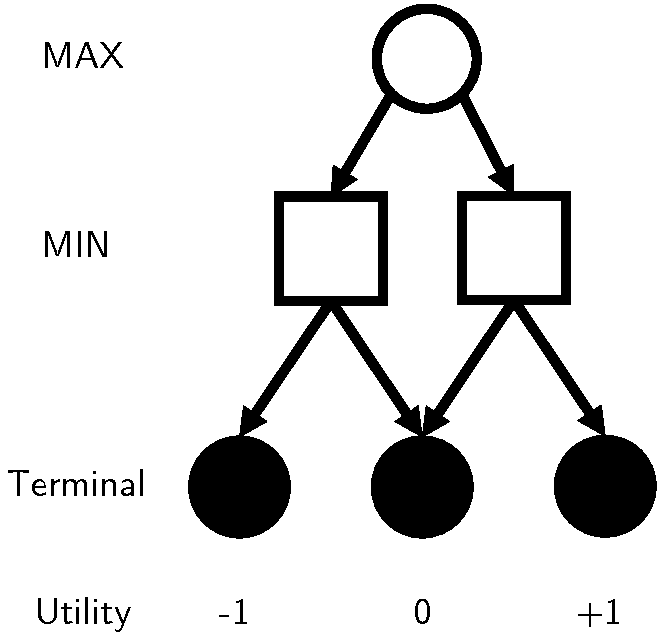
\includegraphics[scale=0.3]{minimax/minimax_step0.pdf}
      \caption{Spielbaum im Ausgangszustand}
      \label{fig:minimax_step0}
    \end{subfigure}
    \begin{subfigure}[b]{0.45\textwidth}
      \centering
      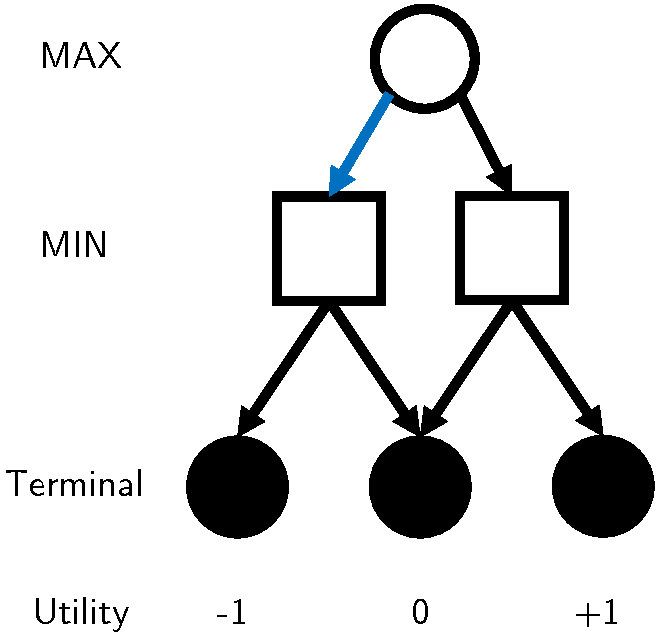
\includegraphics[scale=0.3]{minimax/minimax_step1.pdf}
      \caption{MAX prüft Utility der Kindknoten}
      \label{fig:minimax_step1}
    \end{subfigure}
    \begin{subfigure}[b]{0.45\textwidth}
      \centering
      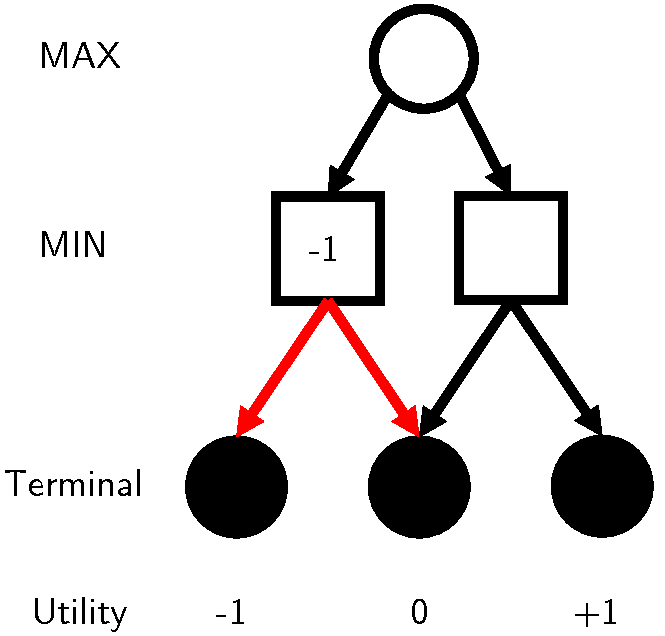
\includegraphics[scale=0.3]{minimax/minimax_step2.pdf}
      \caption{MIN prüft Utility der Terminalknoten und übernimmt kleinste Utility}
      \label{fig:minimax_step2}
    \end{subfigure}
    \begin{subfigure}[b]{0.45\textwidth}
      \centering
      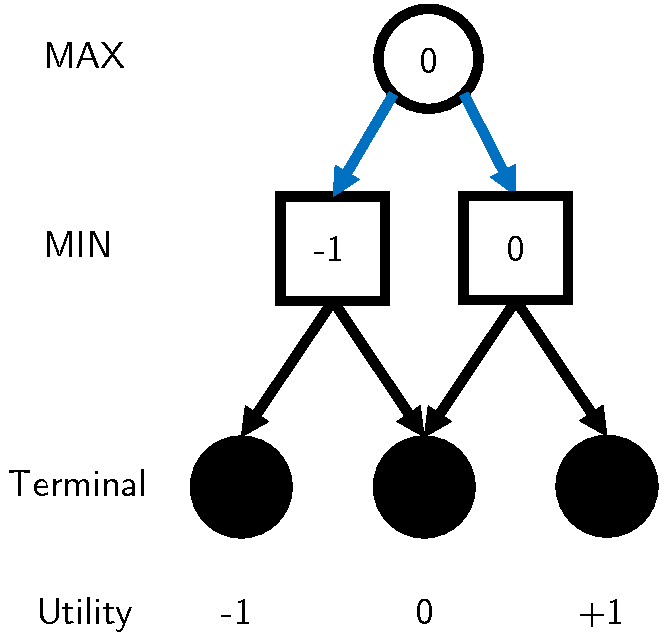
\includegraphics[scale=0.3]{minimax/minimax_step3.pdf}
      \caption{b) und c) werden für rechte Seite wiederholt und MAX wählt größte Utility aus}
      \label{fig:minimax_step3}
    \end{subfigure}
    \caption[Visualisierung des Minimax-Algorithmus]{Visualisierung des Minimax-Algorithmus für ein fiktives Zweispieler-Nullsummenspiel in vier Schritten. Knoten des maximierenden Spielers (MAX) sind Kreise, Knoten des minimierenden Spielers (MIN) Quadrate.}
    \label{fig:minimax_example}
\end{figure}

{\centering
\begin{minipage}{0.60\textwidth}
\begin{algorithm}[H]
\SetAlgoLined
\DontPrintSemicolon
\SetKwFunction{KwMinimax}{Minimax}
\SetKwProg{Fn}{Function}{:}{}
\Fn{\KwMinimax{NODE, PLAYER}}{
    \uIf{NODE is terminal}{
        \KwRet{utility assigned to NODE}
    }
    \uElseIf{PLAYER is maximizing player MAX}{
        \ForEach{child of NODE}{
            \KwMinimax{CHILD, MIN}\;
        }
        \KwRet{maximal CHILD utility}
    }
    \Else{
        \ForEach{child of NODE}{
            \KwMinimax{CHILD, MAX}\;
        }
        \KwRet{minimal CHILD utility}
    }
}
\textbf{end function}

\caption{Pseudocode Minimax-Algorithmus}
\label{algo_minimax}
\end{algorithm}
\end{minipage}
\par
}


Da manche Knoten in Spielbäumen durch unterschiedliche Zugfolgen erreicht werden können, kann der Minimax-Algorithmus durch eine Transposition table (\dt Zugumstellungs-Tabelle) erweitert werden.
Bei diesen werden Informationen zu Knoten in einer Lookup-Tabelle hinterlegt, sodass direkt auf diese zugegriffen werden kann. \cite[S. 651]{millingtonArtificialIntelligenceGames2009}, \cite[S. 22]{slateCHESSNorthwesternUniversity1983}, \cite[S. 807]{greenblattGreenblattChessProgram1988}
Der Name Transposition table leitet sich vom Schach ab, bei dem unterschiedliche Spielzüge, um einen gleichen Zustand zu erreichen, als Transposition (dt. Zugumstellung) bezeichnet werden \cite[S. 651]{millingtonArtificialIntelligenceGames2009}. 
Andere Vereinfachungen und Erweiterungen des Minimax-Algorithmus, wie beispielsweise \gqq{Negamax} oder Alpha-Beta-Pruning \cite[S. 115]{ertelIntroductionArtificialIntelligence2017} werden in dieser Arbeit nicht betrachtet.

